\documentclass[sigplan,10pt]{acmart}
%\documentclass{article}
\usepackage{graphicx}
\usepackage[caption=false]{subfig}
\usepackage{amsmath}
\usepackage{amssymb}

\title{Expos\'{e}: Leveraging Mathematical Structure in Software Synthesis}
\author{Andr\'{e}s Goens}
\begin{document}
\date{}
\begin{abstract}
The trend is clear: Computing systems of the future will consist of heterogeneous multicores. While this allows for maximal computational efficiency, these systems are extremely difficult to program.
A family of methods that is commonly used to program heterogeneous multicore systems is called \emph{software synthesis}.
It consists of using an abstract representation of the application, which allows to analyze and determine an optimal execution, leveraging heterogeneous resources.
The software synthesis problem has many different subproblems, pertaining the representation of applications and architectures, the recording the behavior of an execution and deciding how to best execute a particular application in an architecture.
Each of these subproblems exhibits much structure, which can be captured in precise mathematical terms. In this thesis we aim to identify, describe and leverage this mathematical structure in different subproblems of the software synthesis process.
This would allow to improve the programmability of heterogeneous multicores, bridging the productivity gap for developers.

\end{abstract}

\maketitle
%\tableofcontents

\section*{Introduction}
%End of moore's law:
Since the invention of the semiconductor, the capacity and performance of computing systems has enjoyed a nearly exponential growth over time. Historically, it has doubled roughly every $1 1/2$ years, an observation which is commonly associated with Moore \cite{schaller1997moore}.
While this trend continues roughly until today, in terms of the number of semiconductors in a computer, the capacity and speed of computing systems has been unable to keep up. It is likely that we are reaching more fundamental barriers, where the laws of physics prevent our
current methods to produce event faster systems. 

%Trend: heterogeneous multicores
Fortunately, we still seem far from reaching the limits of our own ingenuity. In terms of hardware, the trend is clear: The computing systems of the future will consist of heterogeneous multicores. Multicores allow to leverage the technological advances in semiconductors to 
increase the computing power of systems by exploiting parallelism in computation. The heterogeneity of said systems, on the other hand, allows to design units specialized for a particular type of processing, instead of relying solely on general-purpose processors.
While this specialization can have a tremendous impact in the computation speed for some problems, it usually has an even greater impact on energy efficiency, which is arguably even more valuable today.


%problem: programming heterogeneous multicores?
With novel systems come novel problems. While heterogeneous multicores are, in principle, an ideal solution to the complex requirements of today's applications, they come with an equally exceptional challenge.
Programming heterogeneous multicores is difficult. It involves partitioning the required computation into appropriate steps. These steps, in turn, might execute differently well in the various hardware resources on the system,
which might itself depend on the concrete data being processed.
On the other hand, systems incur in significant time and energy costs by transfering data between resources.
To efficiently execute a calculation thus involves orchestrating which steps to execute when and where, a highly non-trivial problem which completely dissapears in the traditional, single-core case.

%a solution: software synthesis
Several approaches have been put forward to deal with these issues.
In particular, a family of promising methods that is commonly used to program heterogeneous multicore systems is called \emph{software synthesis}\cite{bhattacharyya2012software,sgroi1999synthesis}.
It consists of using an abstract, functional representation to describe the application, commonly in the form of a graph. Using this representation,
decisions for mapping the different parts of the application to resources in the architecture, as well as scheduling the execution are taken. These decisions commonly involve static strategies,
but can also include dynamic decisions at run-time. Finally, code is generated using these decisions, such that it might leverage the heterogeneous resources in the architecture.

%many sub-problems in software synthesis: code partitioning/representation of algorithms, tracing/trace analysis, mapping/scheduling, code generation
This software synthesis process, thus, involves several different sub-problems that have to be solved.
The question of how to partition an application and represent it abstractly, particularly, in form of a graph that represents logical dependencies in the application, is a highly non-trivial one.
Assuming such a graph representation, the behavior of the application has to be analyzed.
A general analysis would require, among others, solving the halting problem.
Thus, many common approaches make do with a trace-based approach, where the analysis is restricted to a particular execution, or a set of executions.
Finally, the decision problems of mapping and scheduling involve the knowledge gained from the sub-problems above to consider an exponentially growing number of possibilities and selecting a near-optimal one.

%Problems have mathematical structure! Graph structure of code, traces: monoid, redundancy,  mapping/scheduling (e.g. symmetries, distances)
By virtue of their inherent properties, these problems exhibit a large amount of structure, which can be described and exploited with precise mathematical structures.
The simplest example is the abstract representation of applications.
Using the mathematical structure of directed graphs, properties of the application can be deduced from graph-theoretic principles and graph algorithms can be leveraged for efficiently analyzing these abstract representations of applications.
Similarly, the sets of execution traces of an application can be considered as part of a monoid, usually called the trace monoid. They also have information-theoretic properties that correspond to the relationship between the application and its trace.
The space of mappings, on the other hand, while it grows exponentially, also exhibits much structure. Symmetries in the architecture and application induce symmetries in the mapping space, which can effectively reduce the amount of possibilities to be explored.

%thesis: identify and leverage this mathematical structure to improve software synthesis!
In order to feasibly solve the problems arising in software synthesis and program the heterogeneous manycores with their ever-growing complexity, we must identify and exploit these mathematical structures. The goal of this thesis is to identify and precisely describe 
the mathematical structure in the different subproblems in software synthesis. Then, using the identified structure, we will propose improvements to the state-of-the-art solution methods in order to leverage the mathematical structure inherent in the problems.


\section{The Software Synthesis Problem}

%General software synthesis too broad: concentrate
The term software synthesis covers several different concrete problems, with different abstract representations of applications or architectures.
While the aim of this thesis is to keep the approaches as general as possible, to cover as many variants as possible, concrete instances still have to be considered.
In the following, we will describe the software synthesis problem for executing Kahn Process Networks~\cite{kahn74} in heterogeneous architectures, as described in~\cite{castrillon14_springer}.
While this is not the most general instance of software synthesis, it provides enough generality to understand most concepts, while serving as a concrete instance to implement and test the improvements on real examples.
Throughout the thesis we will use this instance as the basis for the software synthesis problem, and will explicitly discuss, when generality is possible, how this is the case and how to leverage it.

\subsection{Kahn Process Networks}

The problem of mapping KPN applications to heterogeneous hardware involves abstractions at different levels, as depicted in Figure~\ref{fig:problem}.
At the \textbf{application} level, programs are described using the KPN model. In this model, applications are partitioned into
different \emph{processes}, which encapsulate the different parts of the computation. These processes are not isolated;
they communicate by exchanging data. In the KPN model this is abstracted by defining communication \emph{channels}
between processes that act as unbounded FIFO buffers. The Kahn \emph{process network} is the resulting system, usually formalized as a graph 
with processes as nodes and channels as edges.

 \begin{figure}
 	\centering
 	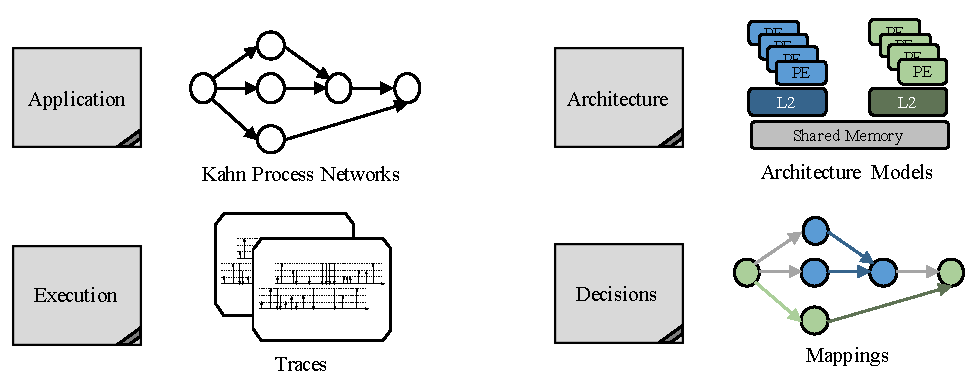
\includegraphics[width=.48\textwidth]{figures/problem.pdf} 
 	%	\vspace{-5mm}
 	\caption{An instance of software synthesis: Mapping KPN applications to heterogeneous architectures.}
 	\label{fig:problem}
 		\vspace{-3mm}
 \end{figure}

The structure offered by KPNs has several advantages. One of these comes at the \textbf{execution} level. 
From its semantics, KPN applications are deterministic~\cite{kahn74}. 
That is, the process network will always produce the same results given the same input.
In particular, the results are independent of the execution order of the processes and individual timings,
provided no artificial deadlocks are introduced when restricting the sizes of the FIFO buffers.
This fact can be utilized to create program traces of a KPN application that are independent of the execution,
capturing the behavior of the execution at a high abstraction level.

Abstractions are also required for describing the hardware \textbf{architecture}.
To this end, an architecture is described as a set of \emph{processing elements} (PEs) and \emph{communication resources}.
The latter is an abstraction for any way data can be shared between processes residing on one or several PEs. 
These range from simply shared memories, and local scratchpads for single PEs, to specialized resources like hardware-FIFOs.
Actual hardware architectures, and the libraries used (or operating system, if applicable), are much more complex than this.
However, there is no simple abstraction that allows to capture all these details in a straightforward manner, 
which is why different frameworks use different such abstractions.

Using these models, \textbf{decisions} are made for deploying the applications onto the hardware. At this level,
one also uses abstractions. As is canonical from the application description, processes are mapped to PEs, 
and the communication channels between them to hardware resources. It is also common to distinguish between the mapping of
processes to PEs and the scheduling at runtime.
In this thesis, we limit ourselves to scheduling within a single PE when several processes have been mapped to it.
There are additional decisions that have to be taken in this context, like \emph{buffer sizing}, where the sizes of the
FIFO buffers have to be chosen. 

The problem of mapping KPN applications to heterogenous hardware, as studied in this thesis, is that of
finding a mapping of processes to PEs and of channels to communication resources. 
This mapping should be optimal or at least near-optimal in some sense for a particular execution, which is captured in the form of a trace.
Optimality can be defined in different ways, like execution time, energy consumption or resource usage (while respecting a particular real-time bound).

A concrete implementation aimed at solving this precise problem is realized in the commercial software suite SLX, which is based on the MAPS framework~\cite{maps08,castrillon14_springer}
The application is written as a KPN in an extension to the C programming language, CPN~\cite{sheng2014_cpn}. Similarly, an architecture description is given as an xml file.
The tool uses novel methods for performance estimation to extrapolate the performance of the execution in the target architecture~\cite{TRETS_eusse14}, generate a mapping with heuristics~\cite{castrillon2012,castrillon_industrial_informatics} and produce executable code.
This thesis will use SLX tools to evaluate approaches and improvements, whenever applicable.

Figure~\ref{fig:synthesisflow} shows an abstract representation of the software synthesis flow, as described above and implemented in SLX.
\begin{figure}[h]
	\centering
	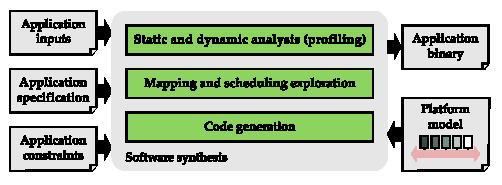
\includegraphics[width=0.45\textwidth]{figures/synthesisflow.pdf}
	\caption{Abstract view of a software synthesis flow}
	\label{fig:synthesisflow}
\end{figure}


\section{Current Status}

In the following section we will describe our previous work leveraging mathematical structure in software synthesis. For space reasons, this exposé cannot go in-depth in the mathematical structures and the methods devised to leverage them.
Instead, the aim of this section is to give an overview and present results, to show how, in principle, mathematical structure can be leveraged to improve solutions to the software synthesis problem.

\subsection{Symmetry in mappings}\label{sec:symmetries}

The mapping of applications described by an abstract, graph-based representation to heterogeneous architectures exhibits many symmetries, in practice~\cite{goens_iess15,goens_taco17}. Consider the example shown in Figure~\ref{fig:symmetries_idea}.
To illustrate the principle, the figure depicts a simple homogeneous many-core with a network-on-chip interconnect. Due to the homogeneous structures of the platform, it is intuitive to see that the two leftmost mappings of tasks to processing nodes should lead to basically the same execution behavior, 
if we neglect effects like process variation or aging.
Conversely, we can expect the third, rightmost mapping to have a different execution behavior, since the communication paths are different than in the first two. 
In the presence of heterogeneous resources, such an analysis becomes less obvious.
Even more so with complex network topologies, in architectures with hierarchical structure, when optimizing for different objectives, or when all these are combined.
\begin{figure}[h]
	\centering
	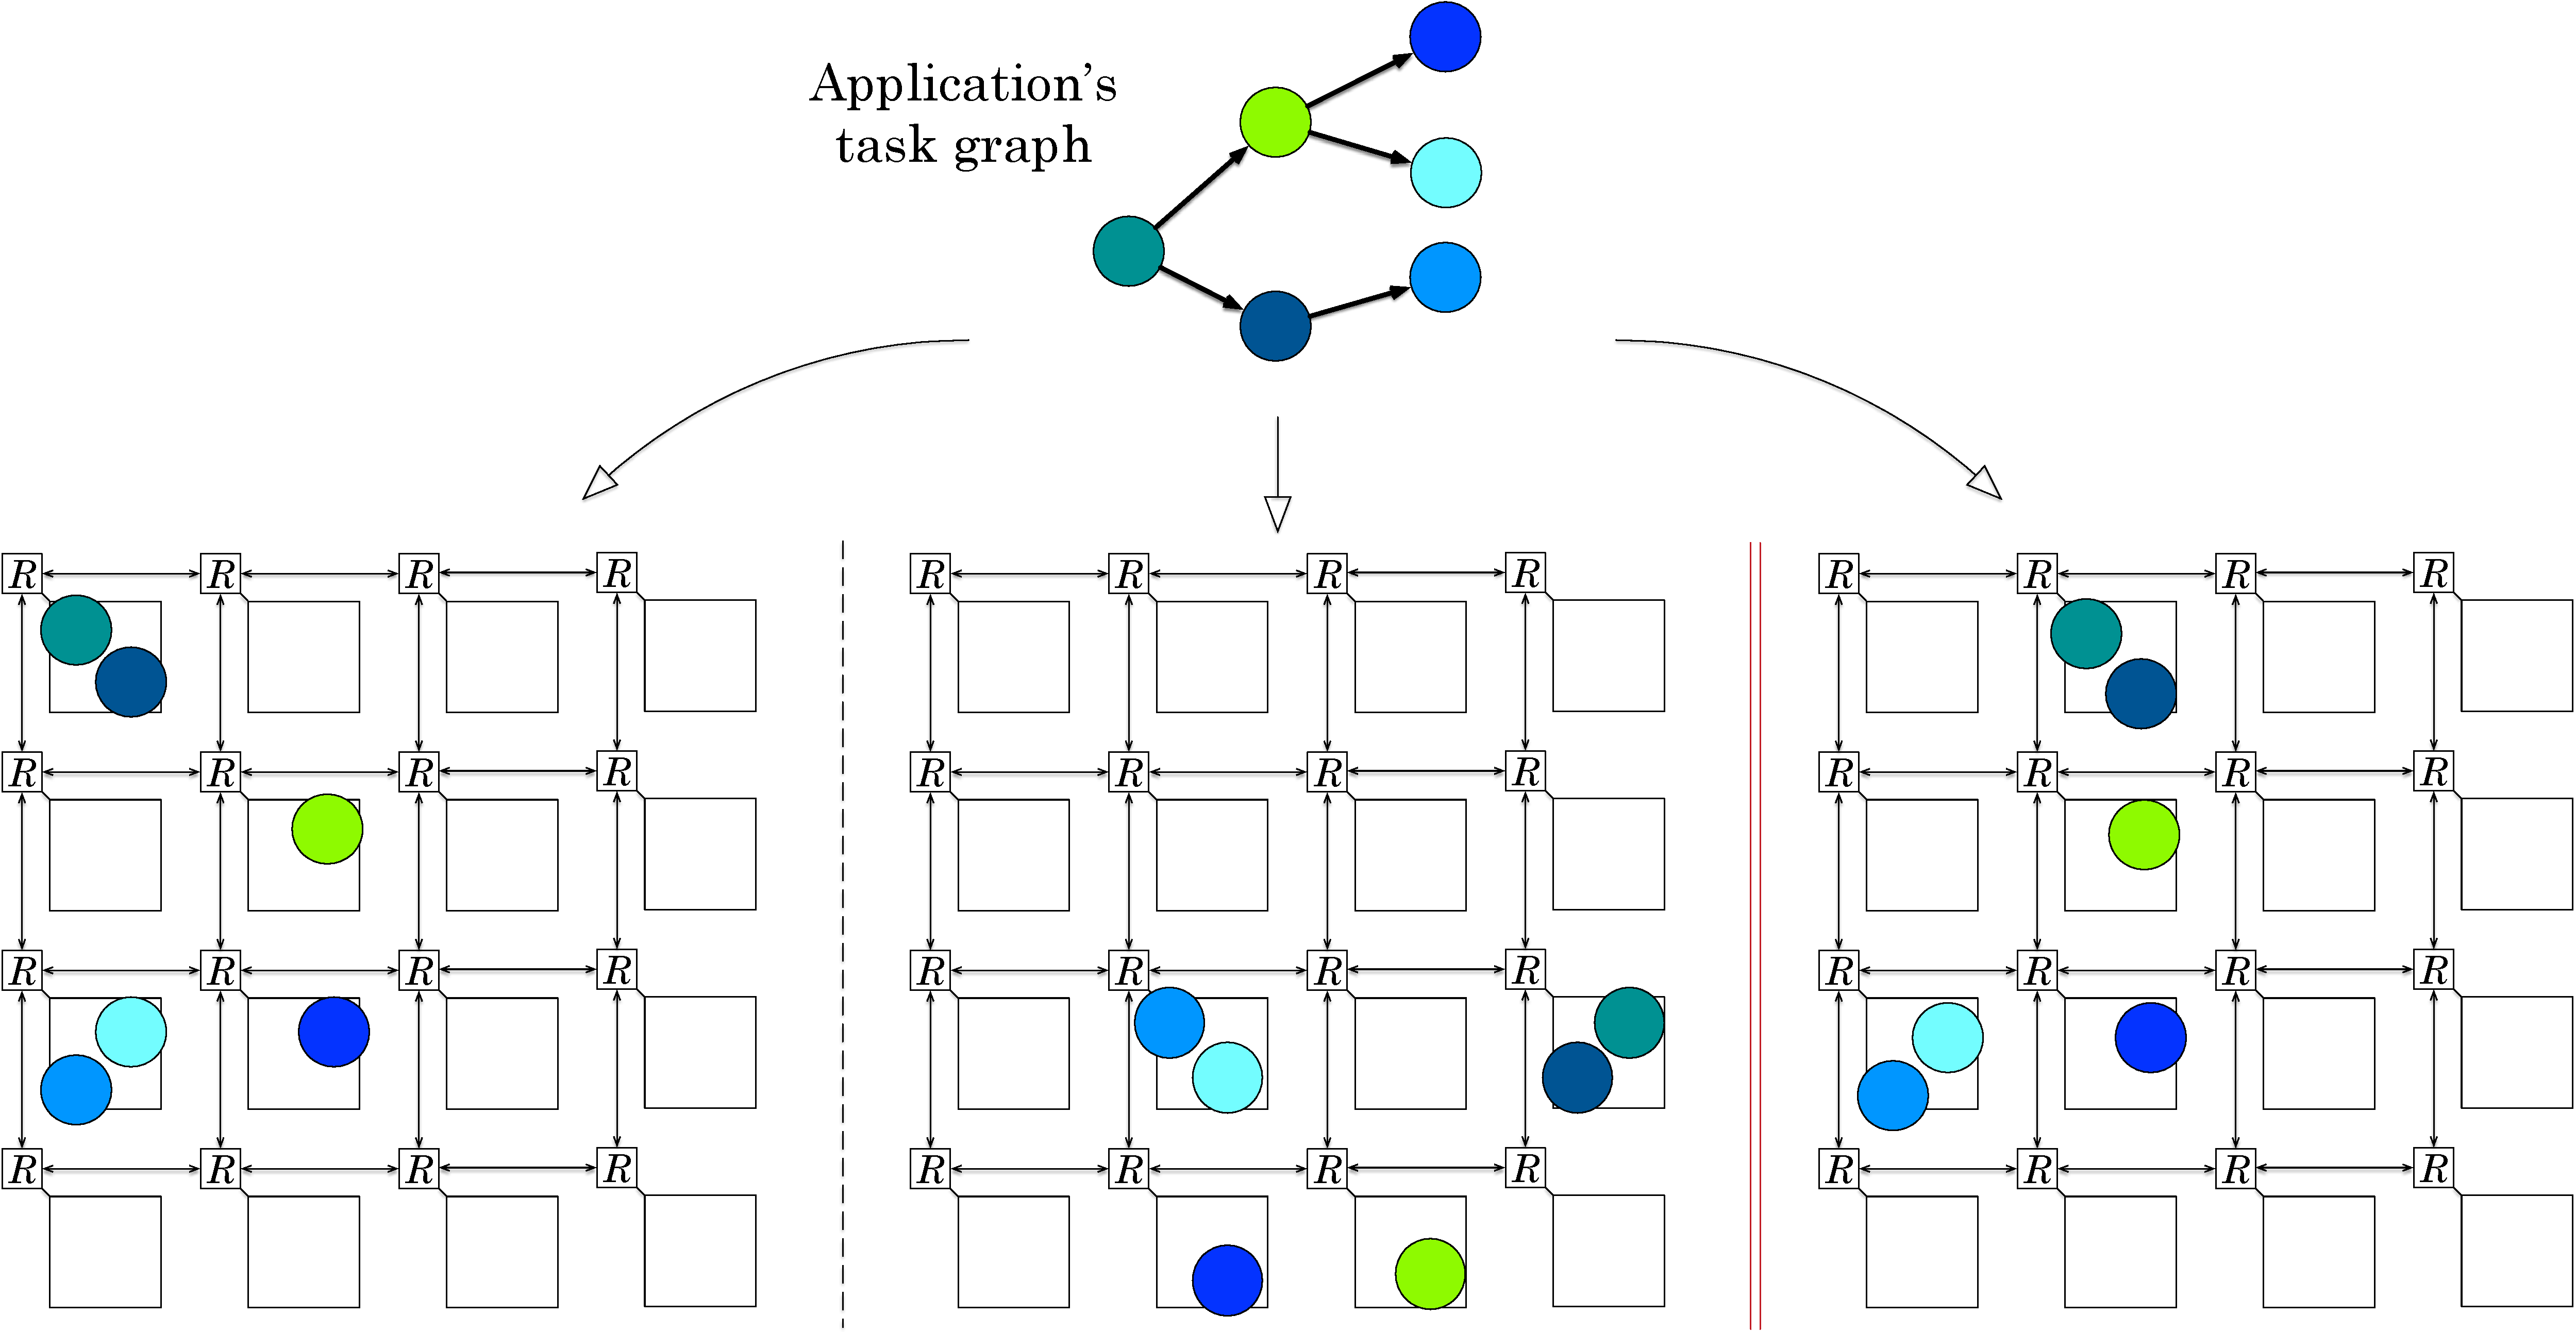
\includegraphics[width=0.45\textwidth]{figures/SymmetriesIntro.pdf}
	\caption{Illustration of symmetries. The two left mappings are equivalent, while the one on the right is not.}
	\label{fig:symmintro}
\end{figure}


\subsubsection{Mathematical Structures}

In order to describe mappings of KPNs to heterogeneous architectures mathematically, we need a mathematical description of the architecture and of the KPN. 
A KPN has a very precise mathematical definition, for its semantics, as can be found in the original paper by Gilles Kahn~\cite{kahn74}. However, for this exposé the semantics are not essential. Thus, it suffices to consider them as a directed
graph $K = (V_K,E_K)$ with a vertex set $V_K$ of processes, and an edge set $E_K$ of channels. Processes can execute concurrently and communicate solely through the channels, which can be though of as FIFO buffers.

For describing architectures, our approach uses a structure called the \emph{architecture graph} to capture the architecture topology~\cite{castrillon2012}. This multigraph $A = (V_A, E_A)$ has a node $v \in V_A$ for every processing element (PE) in the architecture.
A function $l$ labels all the PEs in $V_A$ with their PE type in heterogeneous architectures.

For every communication resource $r$ that can be used between two PEs $v_1, v_2 \in V_A$, the architecture graph has an edge $(v_1,v_2,r) \in E_A$, where $r$ is a label for that communication resource.
As an example, consider the Exynos architecture, as illustrated in Figure~\ref{fig:exynos}.
It has eight ARM PEs, following the big.LITTLE\texttrademark~principle, with four ARM Cortex A7 PEs (the ``little'' ones) and four ARM Cortex A15 PEs (the ``big'' ones). 
For it, the architecture graph of the Exynos architecture is depicted in Figure~\ref{fig:arch_graph}. The labels for the different communication resources and PE types can be seen in the colors of the edges and nodes in the graph.

This architecture graph can be readily obtained from the architecture description in the SLX Tool Suite, or any similar description which includes the structure of the hardware architecture. 
In fact, the objective of the architecture graph is to allow us to capture, in a mathematical object, precisely this \textbf{structure}: the topology, PE types and the communication resources available.
Only by using the formal nature of this architecture graph we can extract the symmetries of the architecture algorithmically, i.e., in an automated fashion.


\begin{figure*}[t!]
%
	\subfloat[The heterogeneous Exynos architecture.\label{fig:exynos}]{
     \begin{minipage}[b]{0.41\textwidth}
	\centering
	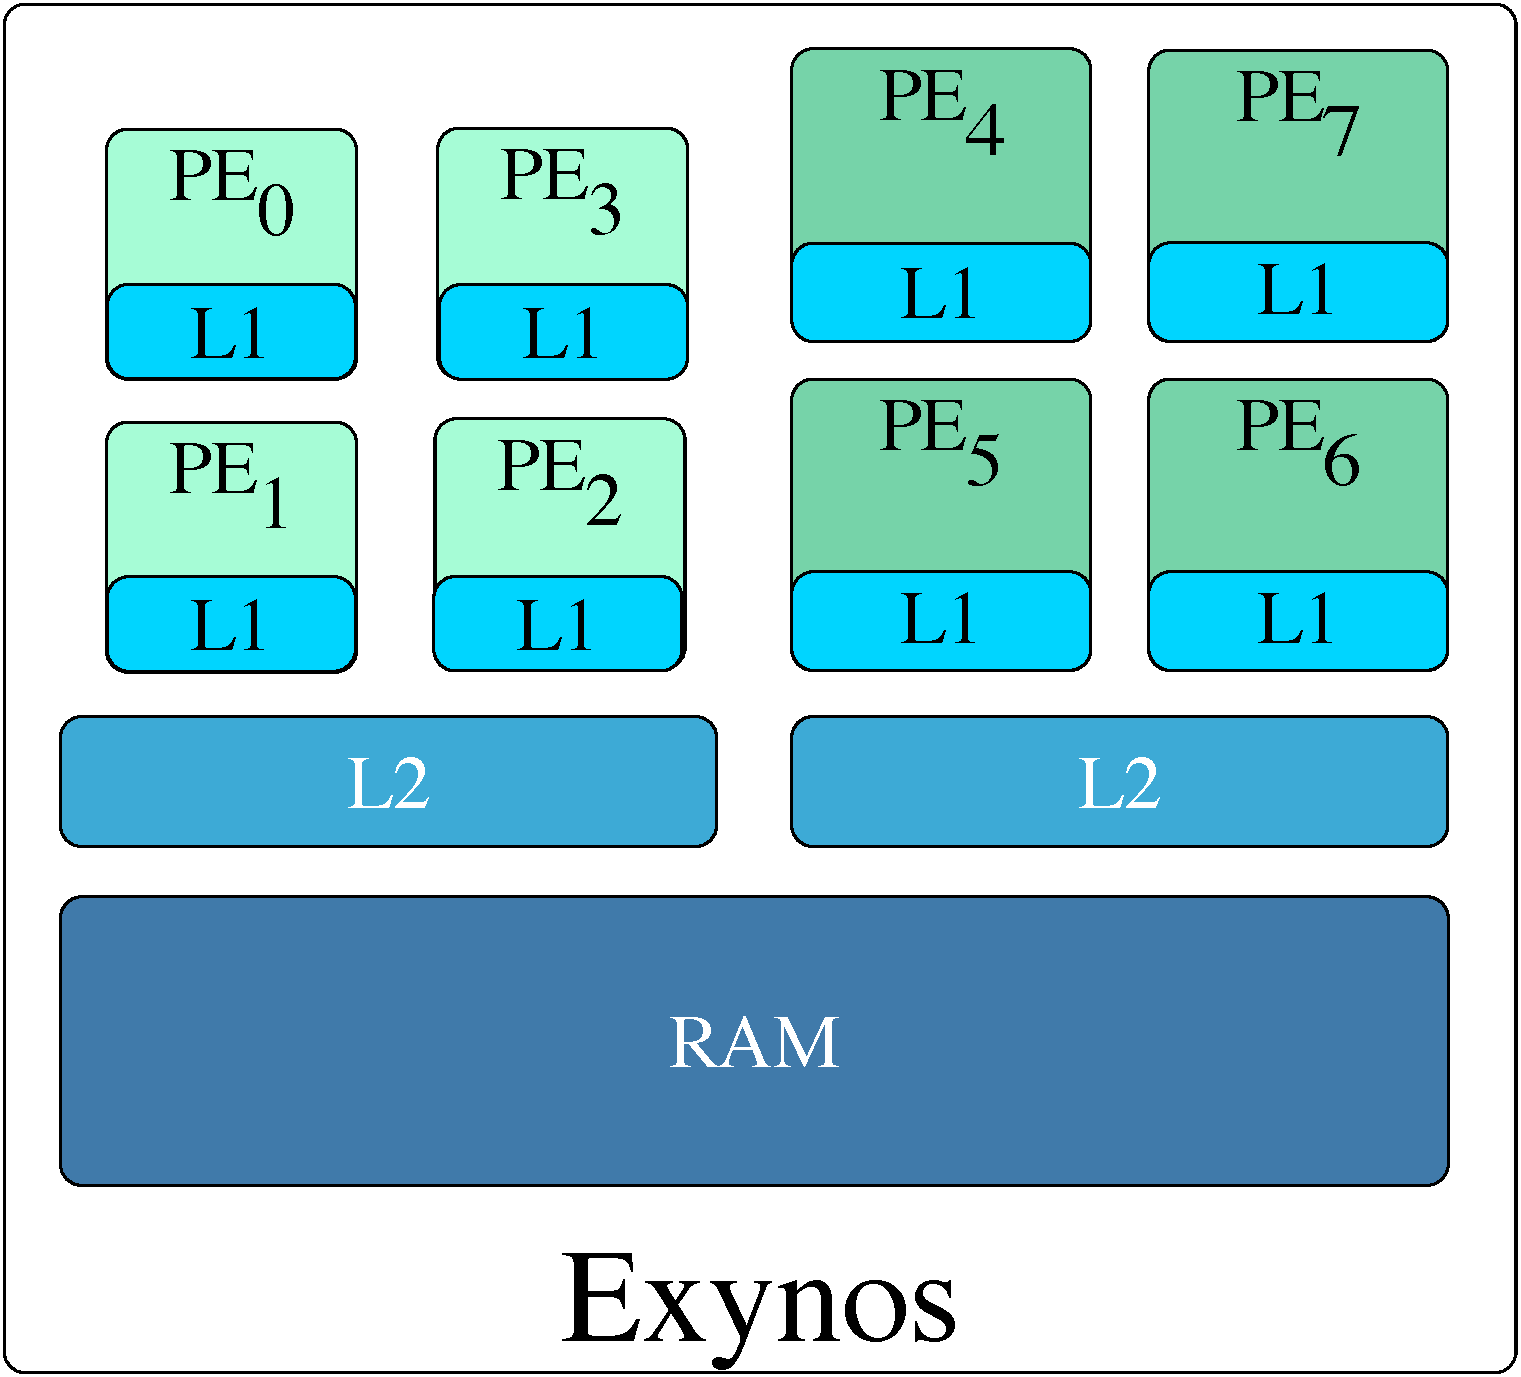
\includegraphics[width=0.8\textwidth]{figures/exynos.pdf}
	%
	%
		\end{minipage}
	}
	\hfill
	%
	\centering
	\subfloat[The architecture graph of the Exynos.\label{fig:arch_graph}]{
		\begin{minipage}[b]{0.54\textwidth}
	\centering
	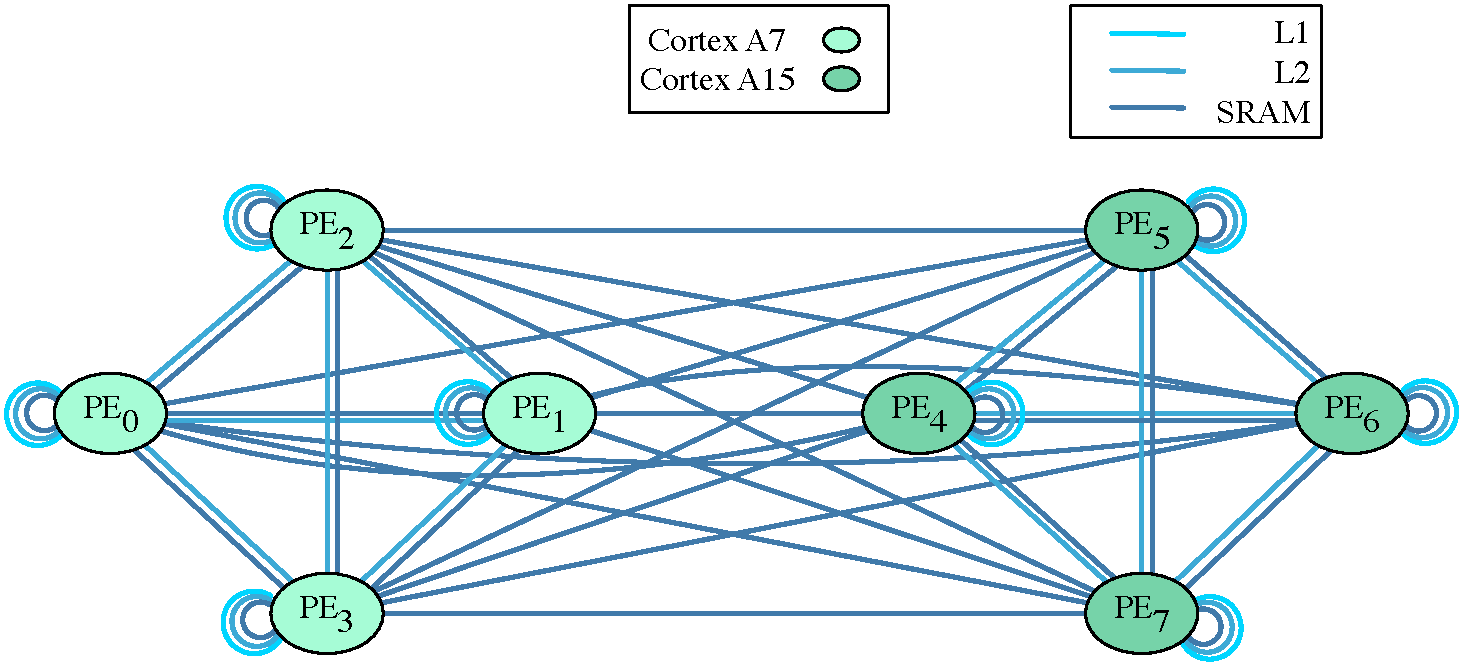
\includegraphics[width=0.94\textwidth]{figures/exynos_archgraph.pdf}
	%
	%
		\end{minipage}
	}
	%
	\caption{An example architecture and its corresponding architecture graphs.}
	\label{fig:actionsm1}
 \end{figure*}
 
A mapping of a KPN $K$ to an architecture with architecture graph $A$ is thus simply a morphism of graphs $m: K \rightarrow A$. The condition that edges from $K$ are mapped to edges from $A$ ensures that FIFO buffers can be realized.
In practice, FIFO buffers and communication resources would have an annotation to their size, and a valid mapping would additional respect these sizing constraints. In this exposé, however, we will disregard these issues for simplicity.

An automorphism $\varphi: A \rightarrow A$ of the architecture graph, i.e. a graph isomorphism respecting labels of $A$ to itself, describes a symmetry of the problem.
Since even heterogenous architectures usually have several identical components, the groups of automorphisms of architecture graphs $A$ are non-trivial~\cite{goens_iess15}.
These symmetries of the architecture induce symmetries on mappings, as illustarted in Figure~\ref{fig:symmintro}.
Similarly, if we know an automorphism from the semantics, it also induces symmetries in the space of mappings. 

In general, however, to capture all symmetries of an architecture that can be exploited, the approach using group theory is not sufficient. 
Consider the NoC-mesh as depicted in Figure~\ref{fig:4x4NoC_inv_semi}. Compare the colored regions in the different depictions of the architecture in the figure.
A computation using only the cores of the blue region to the left should have the same performance values as the one in the blue region to the right, with the transformation implied by the dark-blue arrow:
\begin{align}
\label{eq:partial_4by4}\text{PE}_1 \mapsto \text{PE}_{2}, \text{PE}_{5} \mapsto \text{PE}_{6}, \text{PE}_9 \mapsto \text{PE}_{10}, \text{PE}_{13} \mapsto \text{PE}_{14}
\end{align}
However, this mapping is not an automorphism of the architecture graph corresponding to this mesh.
The fundamental difference between this transformation and symmetries of the automorphism group, like rotations and reflections is that this transformation is only defined on a subset of the four-by-four mesh and cannot be extended to a symmetry of the full mesh.
To accurately describe and leverage symmetries like that depicted in Figure~\ref{fig:4x4NoC_inv_semi}, an approach using the mathematical theory of inverse semigroups is required~\cite{goens_taco17}. For space reasons, this exposé will not delve into the details of this approach.


\begin{figure}[h]
	\centering
	\includegraphics[width=.46\textwidth]{figures/NoC4by4inv_semi.pdf}
	%
	\caption{Partial functions define more symmetries in a 4x4 mesh.}
	\label{fig:4x4NoC_inv_semi}
		%
\end{figure}


%Inverse semigroups

\subsubsection{Reducing design-space exploration}

An application of the symmetries found using the graph formalizations and the theories of groups and inverse semigroups is a reduction of the design-space of mappings. 
To find a good mapping of an application to an architecture, a designer or tool doing software synthesis has to explore an extensive design-space of possible mappings. 
If two mappings are equivalent through symmetries, however, only one of them has to be considered.

Following this principle, we modified a design space exploration framework to leverage the symmetries of the architecture. The design-space exploration uses evolutionary algorithms within the Sesame~\cite{sesame} framework to explore the space of mappings. 
It has a cache which tests if a configuration has been evaluated before, in order to avoid reevaluation.
We augumented this cache with a symmetry-testing improvement, such that it would also stop reevaluation if an equivalent mapping had already been evaluated before, instead of only an identical one.
We tested several applications applications from the signal processing and multimedia domains by mapping on an accurate model of a state-of-the art heterogeneous multicore system, the Texas Instruments (TI) Keystone II. It features 4 ARM Cortex-A15 processing elements and 8 DSPs~\cite{keystone2_whitepaper}. 
The model was adapted~\cite{goens_mcsoc16} from a model of the commercial state-of-art MPSoC compiler from the SLX Tool Suite and confirmed with measurements from hardware~\cite{odendahl2013split}.

\begin{figure*}
	\centering
	\includegraphics[width=0.9\textwidth]{figures/wall_genetic.pdf}
	%
	\caption{A comparison of benchmarks for the improved caching strategy in Sesame. The red bars on top represent the overhead, while the dotted gray line marks the baseline (without symmetries). }
	\label{fig:genetic_algorithms}
	%
\end{figure*}

We executed the DSE framework with $5, 20, 50$ and $200$ generations for all benchmarks, with five different (fixed) random seeds, repeating each such configuration five times.
It uses an evolution-strategy called $\mu + \lambda$, which we used with fixed populations of size $20$ and with $20$ children.
We measured the overall wall-clock time of the DSE using our improved cache strategy and the conventional cache. Additionally, we
measured explicitly the time spent in symmetry-related calculations in the improved cache. The results are summarized in Figure~\ref{fig:genetic_algorithms}.
It shows the normalized average of the total execution time for all benchmarks, separating the time spent on the DSE from the overhead of the symmetry calculations. 
The difference to the baseline of $1$ is the percentage of time which was saved by avoiding redundant calculations.
The plot shows the overhead is negligible in all cases; indeed, it represents between $0.1-0.2 \%$ of the total execution time across the different benchmarks.
The plot also shows that the improved cache results in a net improvement of the execution time, in spite being a prototype implementation. 
As expected, the effects of symmetry were more visible in explorations with a larger number of generations (and thus, of simulations).

Similarly, we modified an iterative algorithm for minimal resource usage in soft real-time scenarios in SLX. We obtained significantly better resource utilization by considering symmetries, compared to a simple algorithm which does not consider them. 
Compared to a brute-force approach, we obtained a speed-up by a factor of $10$. More details of both usecases, as well as the theory behind the symmetry identification and reduction can be found in~\cite{goens_taco17}.

\subsubsection{Run-time adaptivity}


When designing software for embedded systems, reliability and predictability are usually just as much an asset as raw performance~\cite{edwards2007case,axer2014building,lee2008cyber}.
Today, with the increasing availability of high-performance embedded devices, like the ARM big.LITTLE\texttrademark~platforms~\cite{biglittlewhitepaper} or the many-core Epiphany-based systems~\cite{olofsson2016epiphany}, the lines between commodity, high-performance and embedded system devices and ecosystems are becoming increasingly blurred.
Several modern embedded systems interact with the environment in a plethora of ways at the same time.
This increases the unpredictability of software execution, since the workload of the system depends on many different and independent applications~\cite{lee2008cyber}.
%This is especially relevant when the system is designed to interact with the physical environment, be it a person watching a video on a tablet device, an LTE decoder on her phone
%or even the pacemaker that keeps her heart beating. For (hard) real-time systems, like the pacemaker, performance guarantees are non-negotiable and should be met at any cost.
%On most other applications, though, a reliable performance is desirable only to a reasonable cost. 
%This is understandable: a missed frame is usually not as disastrous as a missed heartbeat.

\begin{figure}[t]
	\centering
	\includegraphics[width=0.40\textwidth]{figures/tetris.pdf}
	\caption{The basic idea behind TETRiS}
	\label{fig:tetris_idea}
%  \vspace{-3mm}
\end{figure}

In several cases, the traditional notions of real-time software do not always apply anymore: many applications are too complex and variable, yet not critical enough for a rigorous worst-case execution-time analysis and verification.
Consider a modern mobile phone. It has to keep several background processes running for the normal functioning of the phone, while being used for high-quality video playback. If then, a high-performance request 
gets scheduled, e.g., from a bluetooth device which wants to do simultaneous location and mapping using the phone, it would be ideal to keep the same performance for the other tasks, without changing the user experience.
To ensure this, the allocation of resources might need to be adapted dynamically, while keeping the performance equal.
We need approaches that ensure an execution that is predictable and efficient on average, even in the presence of dynamic changes in the system's load.

A large body of research has been dedicated to programming applications for these modern embedded systems~\cite{eker2003taming,thiele2007mapping,maps08,pimentel2006systematic,nikolov2008daedalus}. Common approaches structure the application in an abstract way, and can thus make
decisions based on these abstract models of computation. Usually: how to partition the application code, and where and how to schedule this partitioned code. The ``where'' question is sometimes also called \emph{mapping}.
In particular, it is a common practice to use static mapping and scheduling strategies at compile-time to obtain predictable outcomes~\cite{bekooij2004predictable}.

However, flows considering static resource allocation and concentrating on a single application struggle when dealing with multiple applications.
The estimated performance of an application does not consider other applications that will compete for system resources.
This leads to significantly worse and less predictable performance when, at run-time, this isolated view of the application does not hold anymore.
To avoid contention in the communication, hardware support like Network-on-Chip technologies  
or mechanisms at the hardware level to ensure isolation and predictable communication patterns between tasks~\cite{hansson2009compsoc,kumar2008analyzing} are required. 
These concepts, along the lines with the concept of precision timed (PRET) machines~\cite{edwards2007case}, require very specific hardware, not all of which has been embraced by chip manufacturers yet.

We can leverage the same mathematical structure of symmetries to deal with these issues. Instead of considering only one mapping out of a whole equivalence class in the desgin-space exploration at compile-time, we can leverage the equivalence class at run-time.
In this section we present a novel approach to keep applications in their isolated view at the software level, obtaining reliable performance in dynamic multi-application scenarios.
While the methods should produce the best results on precision-timed machines, our implementation also works on off-the-shelf heterogeneous multi-processor system-on-chips (MPSoCs) and is compatible with Linux.
We call our approach the \textbf{T}ransitive \textbf{E}fficient \textbf{T}emplate \textbf{R}un-t\textbf{i}me \textbf{S}ystem (TETRiS).

Figure~\ref{fig:tetris_idea} summarizes the idea of the TETRiS approach. It uses near-optimal static mappings for the isolated applications, as depicted
on the upper side of Figure~\ref{fig:tetris_idea}. Then, it revolves around an innovative strategy for mapping multiple applications by 
identifying and selecting mappings with equivalent performance properties. By using the mathematical structure from the symmetries, it can automatically and precisely identify, at compile-time, classes of mappings that will have the same performance on a system.
Figure~\ref{fig:tetris_idea} shows what would happen when using no strategy at all, which results in a very
inefficient resource distribution, an unpredictable redistribution, as would probably be computed, e.g., by the operating system's scheduler (CFS, the Completely Fair Scheduler, in the case of Linux), and TETRiS, where the structure of the 
mapping is preserved. Since our method leverages the structure of the architecture only, it is agnostic to the mapping strategy and its objectives. By using a strategic precomputation step, this can be done with almost no overhead at run-time. 

We evaluate the TETRiS approach by embedding it into a state-of-the art commercial compiler for multicore systems, SLX~\cite{slx}.
We use it then to execute multiple applications from the signal processing and multimedia domains on a modern heterogeneous architecture.

\subsection{Mapping Algorithms}
The approaches we have outlined so far assume an existing algorithm for mapping and improve it. However, the mathematical structure of the problem can also be leveraged to improve 
\subsubsection{Comparing Algorithms}
%The need for abstract models of architecture
%Metaheuristics > Heuristics, problem: time!
\subsubsection{Design centering}
 %Robust mappings

\section{Planned Work}

In this section we will propose diverse options of other mathematical structures in software synthesis that can be explored, or ways to leverage the ones identified already.

\subsection{Application Graphs}

The structure of the application as a graph is already a well-defined mathematical structure with useful properties.
Not only dataflow graphs, but also task graphs or other dependency graphs all share the property of describing the flow of the algorithm in a graph structure.
This structure can be leveraged for analysis or for transformations.

\subsubsection{Graph transformations}
In dataflow execution models, the dataflow graph is part of the program semantics. By formalizing these semantics, giving them a mathematical structure, a graph transformation can be performed such that it preserves the program semantics.
This can be used to improve an execution by doing I/O-optimizing transformations, or increasing the number of parallel executions when data-parallelism is involved.
We are currently working on \"Yauhau, an engine that transforms dataflow graphs to improve I/O in microservice-based architectures. 

\subsubsection{Graph semantics}
The KPN semantics are usually implemented using the Kahn-MacQueen execution model~\cite{kahnmacqueen}. This model uses blocking reads and writes on communication channels in order to ensure a deterministic execution.
However, the semantics as defined by Kahn~\cite{kahn74} do not require these blocking writes and reads. A model with a non-deterministic execution order, which nevertheless ensures the ordering of channel tokens is thus also compatible with the KPN semantics.
This ``MacQueen Gap'' can be thus leveraged to extract instances of data-parallelism in Kahn Process Networks.

\subsubsection{Graph Symmetries}
As explained in Section~\ref{sec:symmetries}, symmetries at the application (graph) level can be leveraged for mapping just as those for the architecture.
While determining the symmetries for the architecture is straightforward from the architecture graph, the same does not hold for the application.
In order to determine if a graph automorphism of the application graph is indeed a symmetry in the execution, the semantics of the program have to remain unchanged by it. 
This could be verified using compiler technologies.

\subsection{Architectures}
Considering the target architecture or hardware platform is crucial for the software synthesis problem.
In order to effectively rely on the different, possibly heterogenous, components of the system, it is vital to know what these components are and what they are capable of.


\subsubsection{Formal models of architecture}
The architecture and the corresponding architecture graph have a precise mathematical structure, just as the application. However, the applications have well-defined models that include the whole semantics, through the programming languages used to define them.
Architectures, on the other hand, are usually modeled in an ad-hoc fashion. While the architecture graph greatly reflects structural components of the architecture, like its topology, it fails to include several aspects.
In particular, an architecture graph cannot be used to reconstruct the ad-hoc models with the level of detail required by e.g. a simulator.
A formal description of an architecture is also useful for comparing different software synthesis flows~\cite{goens_mcsoc16}.
Such models have already been proposed~\cite{moa}, and in the work of this thesis we plan to study them and leverage them, or improve them if necessary.

\subsubsection{Symmetries}
The work on symmetries, while providing a base for leveraging the symmetries of the architecture, still has much room for improvement. Especially for NoC-based architectures, the time required to calculate symmetries is too high, since general algorithms are used.
In future work we plan to leverage domain-specific knowledge about the possible (and consequently, about the impossible) instances of symmetry semigroups that can arise in software synthesis to greatly improve the algorithms in this application.

\subsection{Traces}
Modern applications are often complex and very dynamic.
Depending on the data, the execution of two instances of the same application might have a very different behavior.
Even if the behavior is more predictable, it has to be captured mathematically in order to leverage its structure.
This is done through execution traces. Traces record different events throughout the execution and annotate them in different ways. Mathematically, the Mazurkiewicz traces capture the structure of these execution logs~\cite{bookoftraces}.

\subsubsection{Multiple Traces}
In order to deal with the dynamic behavior of applications, the behavior of different executions of a single application has to be captured and analyzed.
This includes understanding commonalities of the execution behavior of an application to all inputs, as well as potential differences that might be input-dependent.
This can be directly translated into the language of traces.
For a deterministic model of computation, there is a one-to-one correspondence from input stimuli to execution traces.
Thus, analyzing the different possible execution behaviors is tantamount to an analysis framework for multiple traces.

\subsubsection{Trace Compaction}
Traces describe the behavior of an application while computing a specific input stimulus (data). Often, the structure of the trace depends on the data itself, and might vary significantly, depending on the nature of the application.
If the calculation takes a long time, the trace will reflect this by being large.
Depending on the granularity and informational content of the events in a trace, even relatively small and simple computations can produce traces of a length that makes them impractical for storage and analysis.
However, the informational content, in the sense of the Kolmogorov Complexity, does not necessarily follow this behavior.
In fact, we believe that in most cases, there should be a very limited set of possible traces for a particular application. The set of such traces depends only of the application.
Similarly, in any deterministic model of computation, a trace itself only depends on the application description and the input data set. This very clearly gives bounds on the Kolgomorov Complexity of traces, which favors the hypothesis.
Thus, we believe if we can identify the relationship between the applications and the structure of its traces, we could find ways of describing traces in a compact and efficient fashion. 
This would have direct effects in the usefulness of all methods which are based on trace-analysis, which includes most state-of-the-art heuristics in the field of software synthesis.

\subsubsection{Synthetic Traces}
In order to evaluate the efficacy of methods, as well as to apply learning-based methods, the behavior of many applications in different scenarios is required. 
Obtaining real benchmarks with large amounts of real data is a complex endeavor, which requires several person-years and is far beyond the scope of this thesis. 
An alternative solution is to leverage the informational structure of traces, similar to the methods for trace compaction.
By characterizing the common structure of traces and their relation to the application, we could leverage this structure to generate synthetic traces that describe realistic behaviors.
These synthetic traces would be useful in many scenarios, to test diverse methods or to produce enough data for others.

\subsection{Mapping Algorithms}
A final part of the software synthesis process which we will consider in this work are mapping algorithms.
Two components are involved in finding a mapping to execute an application.
The first issue is to identify objectives, like performance, resource utilization and energy consumption, and be able to determine, or at least estimate, the goodness of a mapping with regards to these objectives.
The second component of a good mapping algorithm is a method for navigating the exponentially-growing space of possible mappings, in order to find which perform best according to the desired objectives.
While the first described represents tremendous challenges and good engineering, here we will concentrate on this second part, since it is where the most mathematical structure of the problem lies. 

\subsubsection{Genetic Algorithms}
A class of algorithms that is well-suited for design-space exploration, such as is the case of mapping, are the so-called genetic algorithms.
In particular, inspired by the biological process of evolution, a subclass of algorithms called evolutionary algorithms (EA) shines by its usefulness in exploring very complex design spaces and finding Pareto fronts for multi-objective optimization.
Evolutionary algorithms have been applied to different instances of software synthesis successfully~\cite{Quan14}. However, existing EA do not fully exploit the mathematical structure of the mapping space.
As part of this work we plan to design EA that better utilize the mathematical structure of the mapping space that we have identified.

\subsubsection{Discrete Design Centering} 
It is very common in software synthesis that the goal of the synthesis is to maximize or minimize one or several concrete objectives.
Sometimes, however, the goal is for a system to continue to work reliably even in unexpected circumstances. Such a system is then said to be robust. 
We have successfully applied the concept of design centering to the mapping problem to find reliable mappings~\cite{hempel2017robust}.
However, in this exploratory work we also neglected much of the structure of the design-space of mappings, such as its discreetness, or a metric structure, i.e. as a metric space, that could be easily derived from an architecture description.
We believe by taking this additional structure into account, we can significantly improve the search methods for robust mappings.

\subsubsection{Compact Mappings}
Similar to the case for robust mappings, on multi-application scenarios, raw performance or energy-consumption are not always the desired goal. If several applications are to share a single system, special care has to be taken to balance the resource utilization of a mapping.
This principle is not only limited to the total amount of system resources utilized, but also usually their position, especially in modern systems with Network-on-Chip technologies.
In order to deal with this, the graph structures of applications and architecture representations can be leveraged to define mappings that are compact, for example.
We plan to utilize the structure described in this exposé to restrict search algorithms to find mappings with good spatial qualities in their resource utilization. This will be useful for increasing security and reliability by restricting or avoid contention on communication subsystems,
as well as an efficient resource utilization to leverage a single architecture for executing different applications dynamically.

\section{Timetable/Workplan}


%\section{Related Work}


\section{Conclusions} 
%\bibliographystyle{ACM-Reference-Format}
\bibliographystyle{abbrv}
\bibliography{expose} 
\end{document}
